\documentclass[11pt,a4paper]{article}

\usepackage[utf8]{inputenc}
\usepackage[T1]{fontenc}
\usepackage{geometry}
\usepackage{amsmath,amssymb,amsthm}
\usepackage{booktabs}
\usepackage[numbers]{natbib}
\usepackage{tikz}
\usepackage[colorlinks=true,linkcolor=blue,citecolor=blue,urlcolor=blue]{hyperref}

\geometry{
  left=2.5cm,
  right=2.5cm,
  top=2.5cm,
  bottom=2.5cm
}

\newtheorem{definition}{Definition}
\newtheorem{theorem}{Theorem}
\newtheorem{proposition}{Proposition}
\newtheorem{remark}{Remark}

\title{\textbf{NRR-Projection: Projection Retention, State Reduction, and Identifiability in Non-Resolution Reasoning}}

\author{
  Kei Saito\thanks{ORCID: 0009-0006-4715-9176} \\
  Independent Researcher, Japan \\
  \texttt{kei.saito.research@gmail.com}
}

\date{March 2026 \\[0.5em]
\textit{Part of the Non-Resolution Reasoning (NRR) research program.}}

\begin{document}
\maketitle

\begin{center}
\textcopyright\ 2026 Kei Saito.
Licensed under CC BY 4.0.\\
\url{https://creativecommons.org/licenses/by/4.0/}
\end{center}

\begin{abstract}
NRR-Phi defined a text-to-state mapping in which multiple admissible interpretations can remain jointly represented rather than being eliminated at the first output step. This paper asks a narrower theoretical question: under what conditions can retaining multiple admissible projections preserve more task-relevant structure than destructive state reduction to a single retained view? We answer this question inside the existing Phi ontology by taking the NRR state itself as the default object of analysis.

We distinguish non-destructive output projection, which emits one interpretation while preserving internal state, from destructive collapse, which removes non-selected alternatives from the retained state. Under a task-conditioned distribution on admissible states, we show that a retained family of projections is at least as informative about the state as any one of its member projections alone. We additionally show that when a projection family is separating on the admissible state set, it identifies distinctions that any non-injective single projection cannot preserve by itself. These results provide a condition-bounded explanation for why premature destructive reduction can be information-disadvantageous.

To connect the theory to existing evidence without overclaiming, we reinterpret already reported NRR-Boundary findings. In particular, provider-by-order sign flips and conditional-first stable improvements are shown to be naturally readable as differences in retained view order and state-flattening behavior. This section is explicitly post hoc and is not presented as a confirmatory test of the theory.

NRR is not an anti-LLM framework. NRR does not replace standard LLM use. NRR optimizes when to commit and when to defer, under explicit conditions.
\end{abstract}

\noindent\textbf{Keywords:} non-resolution reasoning, projection, identifiability, state reduction, information retention, conditional utility

\section{Introduction}
\label{sec:intro}

NRR-Core and NRR-Phi argue that premature fixation can remove useful structure from reasoning trajectories. NRR-Phi formalized this idea by defining a text-to-state mapping in which multiple admissible interpretations remain represented in a single state rather than being collapsed immediately at output time. What remains underdeveloped is the narrower theoretical question of \emph{why} retaining non-resolved structure can be information-advantageous under some conditions.

This paper addresses that question without introducing a new metaphysics of ``hidden meaning.'' The default object of analysis is the NRR state itself. The target claim is correspondingly narrow: destructive reduction to one retained view can remove distinctions that a retained family of admissible projections would preserve. This is not a claim that unresolved states are always better, nor that ambiguity is inherently desirable. It is a condition-bounded claim about information retention, identifiability, and the costs of premature state reduction.

The motivating intuition is familiar from multi-view observation. A single view may flatten distinctions that become recoverable once multiple admissible views are retained together \cite{hartley2004multiple}. In this manuscript that intuition is only motivational. The formal results concern state representations and projection families, not a full claimed identity between semantic interpretation and geometric vision.

NRR is not an anti-LLM framework.
NRR does not replace standard LLM use.
NRR optimizes when to commit and when to defer, under explicit conditions.

\textbf{Series Consistency Statement:}
Unsupported interpretations are never injected at a fixed evidence state, hypothesis-set expansion is evidence-gated, and unobserved possibilities remain explicitly unresolved. In this paper, the evidence state is fixed before analysis, admissible views are taken only over evidence-consistent states, and no gain claim relies on adding unsupported alternatives.

\subsection{Contributions}

\begin{enumerate}
  \item A Phi-internal formalization that distinguishes non-destructive output projection from destructive collapse.
  \item A theorem showing information monotonicity for retained projection families under a task-conditioned distribution on admissible states.
  \item A theorem showing identifiability gain when the retained projection family is separating on the admissible state set.
  \item A cost-bounded proposition clarifying why the framework implies conditional utility rather than universal superiority.
  \item A post hoc reinterpretation of existing NRR-Boundary results as an empirical contact point for the theory.
\end{enumerate}

\section{Relation to NRR-Phi}
\label{sec:phi}

NRR-Phi defines a semantic state instance as
\begin{equation}
S = \{(v_i, c_i, w_i, m_i)\}_{i=1}^{n},
\end{equation}
where multiple admissible interpretations may remain jointly represented. The present paper adopts that state as its default object of analysis rather than introducing a separate privileged semantic object.

This choice matters because projection and collapse are not equivalent in Phi. Phi already permits singular output without destructive internal reduction. We therefore distinguish two operations.

\begin{definition}[Non-destructive output projection]
For an NRR state $S$, a non-destructive output projection $\Pi_j$ emits one output view $y_j$ while retaining the underlying state:
\begin{equation}
\Pi_j(S) = (y_j, S).
\end{equation}
\end{definition}

\begin{definition}[Destructive collapse]
For an NRR state $S$, a destructive collapse operator $C_j$ retains one interpretation-bearing component and removes the non-selected alternatives from the retained state:
\begin{equation}
C_j(S) = S_j.
\end{equation}
\end{definition}

\begin{figure}[t]
\centering
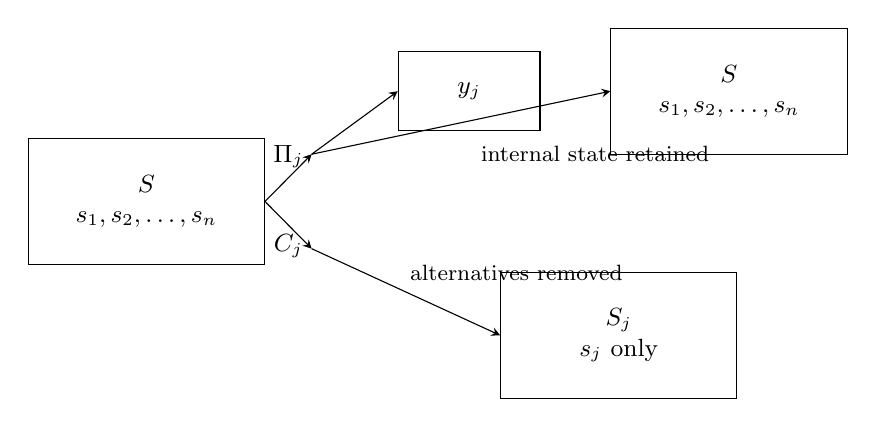
\begin{tikzpicture}[
  x=1cm,
  y=1cm,
  >=stealth,
  every node/.style={font=\small},
  state/.style={draw, rectangle, minimum width=3.0cm, minimum height=1.6cm, align=center},
  outbox/.style={draw, rectangle, minimum width=1.8cm, minimum height=1.0cm, align=center}
]
\node[state] (S) at (0,0) {$S$\\$s_1, s_2, \ldots, s_n$};
\coordinate (u) at (2.1,0.6);
\coordinate (d) at (2.1,-0.6);
\node[outbox] (y) at (4.1,1.4) {$y_j$};
\node[state] (Skeep) at (7.4,1.4) {$S$\\$s_1, s_2, \ldots, s_n$};
\node[state] (Sj) at (6.0,-1.7) {$S_j$\\$s_j$ only};

\draw[->] (S.east) -- (u) node[midway, above] {$\Pi_j$};
\draw[->] (u) -- (y.west);
\draw[->] (u) -- (Skeep.west);
\node[align=center] at (5.7,0.6) {\footnotesize internal state retained};

\draw[->] (S.east) -- (d) node[midway, below] {$C_j$};
\draw[->] (d) -- (Sj.west);
\node[align=center] at (4.7,-0.9) {\footnotesize alternatives removed};
\end{tikzpicture}
\caption{Distinction between non-destructive output projection $\Pi_j$ and destructive collapse $C_j$. Both operate on the same NRR state $S$, but only $C_j$ removes non-selected alternatives from the retained state.}
\label{fig:projection_vs_collapse}
\end{figure}

The theoretical comparisons in this paper are about retained multi-view structure versus destructive collapse $C_j$, not about NRR versus $\Pi_j$. The latter is already compatible with Phi because internal alternatives remain available after output.

\section{Formal Setup}
\label{sec:setup}

\subsection{Evidence state and admissible state set}

Fix an evidence state $E$. Let $\mathcal{S}_E$ denote the set of admissible NRR states consistent with that evidence state. All views, reductions, and comparisons below are restricted to $\mathcal{S}_E$. This restriction prevents gain claims from depending on unsupported interpretation injection.

\subsection{Projection family}

\begin{definition}[Admissible projection family]
Let $\{P_a\}_{a \in A}$ be a family of admissible projection operators on $\mathcal{S}_E$, where each
\begin{equation}
P_a : \mathcal{S}_E \to \mathcal{Y}_a
\end{equation}
returns a partial view of the state.
\end{definition}

Examples include one interpretation choice, one contextual framing, one order-conditioned readout, or one output rendering of the current state. The framework does not require every such view to be equally useful; it requires only that these views be defined over the same admissible state set.

\subsection{Probabilistic reading}

For the information-theoretic result below, we treat $S$ as a random variable distributed over $\mathcal{S}_E$ under a task-conditioned probability measure $\mu_E$. This measure is not part of the ontology of NRR-Phi itself; it is an analytical device for comparing retained views. If this probabilistic setup is considered heavier than needed in a final version, the identifiability theorem in Section~\ref{sec:ident} can stand alone as the primary result.

\section{Main Results}
\label{sec:results}

\subsection{Information monotonicity}

\begin{theorem}[Retained-family monotonicity]
\label{thm:monotonicity}
Let
\begin{equation}
Y_k = (P_{a_1}(S), \ldots, P_{a_k}(S))
\end{equation}
and let
\begin{equation}
Y_1 = P_{a_j}(S)
\end{equation}
for one selected retained view from the same family. Then
\begin{equation}
I(S;Y_k) \geq I(S;Y_1).
\end{equation}
\end{theorem}

\begin{proof}
$Y_1$ is a deterministic function of $Y_k$ obtained by selecting one coordinate. By the data processing inequality \cite{cover2006elements}, mutual information cannot increase under deterministic post-processing, so
\begin{equation}
I(S;Y_k) \geq I(S;Y_1).
\end{equation}
\end{proof}

The theorem does not claim that each additional retained view improves downstream utility in every operational setting. It states only that a retained family cannot be less informative about the state than one of its own retained members alone, before cost terms are introduced.
The contribution of Theorem~\ref{thm:monotonicity} is therefore not the novelty of the inequality itself, but the fact that this comparison is formally safe once projection and destructive collapse are separated inside the Phi ontology.

\subsection{Identifiability under separating families}
\label{sec:ident}

\begin{definition}[Separating family]
A projection family $\{P_a\}_{a \in A}$ is separating on $\mathcal{S}_E$ if for any distinct states $S \neq S'$ there exists some $a \in A$ such that
\begin{equation}
P_a(S) \neq P_a(S').
\end{equation}
\end{definition}

\begin{theorem}[Identifiability gain]
\label{thm:ident}
If $\{P_a\}_{a \in A}$ is separating on $\mathcal{S}_E$, then the full retained family identifies distinctions on $\mathcal{S}_E$ that any non-injective single projection fails to identify by itself.
\end{theorem}

\begin{proof}
If the family is separating, then for any distinct states $S \neq S'$ at least one family member distinguishes them. Hence the map
\begin{equation}
S \mapsto (P_a(S))_{a \in A}
\end{equation}
is injective on $\mathcal{S}_E$. Any single non-injective projection $P_b$ admits distinct states $S \neq S'$ with $P_b(S)=P_b(S')$, so that projection alone cannot identify those distinctions.
\end{proof}

This is the structural core of the argument. Destructive retention of one view can flatten distinctions that a sufficiently rich retained family preserves. In that sense, the theorem is compatible with the broader logic of multi-view learning, where multiple coordinated views can outperform single-view access under appropriate structural conditions \cite{balcan2005pac}.

\subsection{Reduction loss inside Phi}

Even without the probabilistic reading of Theorem~\ref{thm:monotonicity}, a weaker but very safe statement remains.

\begin{proposition}[State-reduction loss]
\label{prop:reduction}
Let $C_j : \mathcal{S}_E \to \mathcal{S}_E^{(j)}$ be a destructive collapse operator. Assume $\mathcal{S}_E$ contains at least one non-trivial state with at least two relevant non-identical alternatives. Then for any state functional $F$ that depends on alternative-sensitive structure, there exist admissible states such that
\begin{equation}
F(S) \neq F(C_j(S)).
\end{equation}
\end{proposition}

\begin{proof}
Take any $F$ that depends on the presence, relation, or weighting of multiple alternatives, and choose a state with at least two relevant non-identical alternatives. By construction, $C_j$ removes non-selected alternatives, so the argument of $F$ changes. Therefore there exist states for which the value of $F$ changes.
\end{proof}

This proposition does not require any hidden-state interpretation. It is entirely internal to the Phi state space and makes clear that destructive collapse can remove structure needed by later operations.

\subsection{Conditional utility}

\begin{proposition}[Cost-bounded utility]
\label{prop:utility}
Let downstream utility be
\begin{equation}
U = G(\text{information retained}) - \lambda \cdot \text{Cost}(\text{retention}),
\end{equation}
with $\lambda > 0$. Assume $G$ is strictly increasing in retained mutual information and $\text{Cost}$ is strictly increasing in the number of retained views. Then there exist regimes in which retained multi-view structure is utility-improving, and regimes in which destructive collapse is utility-improving.
\end{proposition}

\begin{proof}
If discrimination value is high and retention cost is sufficiently low, then by strict monotonicity of $G$ and $\text{Cost}$ the information term dominates and retained multi-view structure improves utility. If latency, memory, or action urgency dominates, then by the same strict monotonicity the cost term can outweigh the retained-information benefit, making destructive collapse preferable. The sign of the utility difference therefore depends on the operating regime.
\end{proof}

This result is necessary for guardrail consistency. The paper does not claim that non-resolution is universally better; it claims that the benefit of retention is conditional on the structure of the task and the cost regime. The form of this tradeoff is also consistent with information bottleneck style reasoning, where retained information is balanced against compression cost rather than treated as unconditionally desirable \cite{tishby1999information}.

\section{Boundary Reinterpretation}
\label{sec:boundary}

The preceding results are mathematical and do not require experiment to stand. However, theory-only presentation can look disconnected from the existing NRR empirical line. To provide a limited empirical contact point, this section reinterprets already reported NRR-Boundary findings through the projection framework.

\textbf{Important scope note:} this section is a post hoc reinterpretation of existing results, not a confirmatory test of NRR-Projection. It shows only that the framework can organize already observed empirical regularities. A direct empirical test would require a separately fixed Projection-specific design.

\subsection{Order-sensitive sign flips}

NRR-Boundary reported ordered-combination cases in which the same operator set changed sign when the order changed. In particular, the pattern \texttt{branch\_conditional} showed sign-flip boundaries on several metrics, with Gemini moving opposite to Anthropic/OpenAI on rows including \texttt{irp\_monotonic\_progress\_rate}, \texttt{misinterpretation\_rate}, \texttt{rework\_cost\_tokens}, and \texttt{stability\_variance}.

These values are reproduced from existing Boundary results, not from new experiments conducted for this paper.

\begin{table}[h]
\centering
\small
\begin{tabular}{p{5.2cm}ccc}
\toprule
Metric & Anthropic sign & OpenAI sign & Gemini sign \\
\midrule
irp\_monotonic\_progress\_rate & $-$ & $-$ & $+$ \\
misinterpretation\_rate & $+$ & $+$ & $-$ \\
rework\_cost\_tokens & $+$ & $+$ & $-$ \\
stability\_variance & $+$ & $+$ & $-$ \\
\bottomrule
\end{tabular}
\caption{Sign-flip cases for \texttt{branch\_conditional}. Data from NRR-Boundary (Saito, 2026); reproduced from existing Boundary results for post hoc reinterpretation, not from new experiments conducted for this paper. Signs reflect rep3 aggregation; rep1 shows zero for some OpenAI rows on these metrics.}
\label{tab:boundary_signflip}
\end{table}

The projection-side reading is straightforward. Order changes which partial view is retained earlier in the trajectory. If a provider's internal behavior makes one early retained view flatten the admissible state more aggressively than another, then downstream quality metrics can reverse direction across providers without any contradiction in the theory. The theory does not predict a universal preferred order; it predicts that different retained-view orders can preserve or destroy different distinctions.

\subsection{Conditional-first stable improvements}

NRR-Boundary also reported that \texttt{conditional\_branch} showed no sign-flip boundary on several practical metrics. It also showed provider-balanced improvements on:
\begin{itemize}
  \item \texttt{irp\_oscillation\_rate}
  \item \texttt{misinterpretation\_rate}
  \item \texttt{rework\_cost\_tokens}
  \item \texttt{stability\_variance}
\end{itemize}

These values are reproduced from existing Boundary results, not from new experiments conducted for this paper.

\begin{table}[h]
\centering
\small
\begin{tabular}{p{4.3cm}cc}
\toprule
Metric & Provider-balanced improvement (mean) & Provider-balanced direction \\
\midrule
irp\_oscillation\_rate & 0.0880 & positive \\
misinterpretation\_rate & 0.0571 & positive \\
rework\_cost\_tokens & 85.5 & positive \\
stability\_variance & 0.0153 & positive \\
\bottomrule
\end{tabular}
\caption{Conditional-first stable cases for \texttt{conditional\_branch} with provider-balanced improvement means. Data from NRR-Boundary (Saito, 2026); reproduced from existing Boundary results for post hoc reinterpretation, not from new experiments conducted for this paper.}
\label{tab:boundary_conditional_first}
\end{table}

The projection-side reading is again condition-bounded. If the conditional view retains discriminative structure that later branching decisions need, then preserving that view earlier can reduce downstream flattening and thereby improve later identification and update stability. This is not a proof of the projection theory. It is a compatible reading of already observed evidence.
This does not elevate conditional-first ordering into a general rule; the stable improvement observed here is specific to the metrics and providers in the Boundary dataset.

\section{Limits and Non-Claims}
\label{sec:limits}

This paper makes several explicit non-claims.

\begin{itemize}
  \item It does not claim that unresolved states are always better.
  \item It does not claim that ambiguity itself is inherently good.
  \item It does not claim that visual parallax and semantic non-resolution are fully identical systems.
  \item It does not claim that entropy alone measures practical usefulness.
  \item It does not claim that unsupported interpretations may be added for the sake of richness.
  \item It does not equate non-destructive output projection with destructive collapse.
\end{itemize}

Theorems~\ref{thm:monotonicity} and~\ref{thm:ident} show structural facts about retained view families and state distinguishability. They do not, by themselves, determine the best operational policy for every system. That choice depends on cost, latency, memory constraints, and the risk associated with delayed versus premature commitment.
The separating condition in Theorem~\ref{thm:ident} is a sufficient condition for identifiability, not a claim that separating families are routinely available in all operational settings.

The Boundary reinterpretation section is especially limited. Because it is post hoc, it cannot serve as a confirmatory test of the theory. A future empirical test would need to manipulate retained-view number, retained-view order, or collapse timing under a fixed protocol designed in advance for Projection-specific hypotheses.

\section{Conclusion}
\label{sec:conclusion}

This paper isolates one narrow theoretical contribution within the NRR program. Working entirely inside the ontology already defined by NRR-Phi, it shows why destructive reduction to a single retained view can remove distinctions that a retained family of admissible projections would preserve. The core result is not that non-resolution is universally superior. The result is that information retention and identifiability can favor non-destructive retention under some conditions, while other regimes rationally favor collapse.

The practical role of this paper is therefore foundational rather than replacement-oriented. NRR-Core defined the program, NRR-Phi defined the state machinery, and NRR-Projection explains one reason why premature destructive reduction can be costly. Existing Boundary results provide a compatible empirical contact point, but a direct confirmatory test of the present theory remains future work.

\begin{thebibliography}{9}

\bibitem{saito2025nrr}
K.~Saito.
\newblock Non-resolution reasoning.
\newblock arXiv preprint arXiv:2512.13478, 2025.

\bibitem{saito2026phi}
K.~Saito.
\newblock NRR-Phi: Text-to-state mapping for ambiguity preservation in LLM inference.
\newblock arXiv preprint arXiv:2601.19933, 2026.

\bibitem{saito2026boundary}
K.~Saito.
\newblock NRR-Boundary: Same operators, opposite effects by provider and order.
\newblock Available at \url{https://github.com/kei-saito-research/nrr-boundary}. Manuscript and data publicly available, 2026.

\bibitem{cover2006elements}
T.~M. Cover and J.~A. Thomas.
\newblock \emph{Elements of Information Theory}.
\newblock 2nd edition, Wiley-Interscience, 2006.

\bibitem{tishby1999information}
N.~Tishby, F.~C. Pereira, and W.~Bialek.
\newblock The information bottleneck method.
\newblock In \emph{Proceedings of the 37th Annual Allerton Conference on Communication, Control, and Computing}, pages 368--377, 1999.

\bibitem{balcan2005pac}
M.-F. Balcan and A.~Blum.
\newblock A {PAC}-style model for learning from labeled and unlabeled data.
\newblock In \emph{Proceedings of the 18th Annual Conference on Learning Theory (COLT)}, pages 111--126, 2005.

\bibitem{hartley2004multiple}
R.~Hartley and A.~Zisserman.
\newblock \emph{Multiple View Geometry in Computer Vision}.
\newblock 2nd edition, Cambridge University Press, 2004.

\end{thebibliography}

\end{document}
